\subsection{New Optimization Strategy}
We introduce three levels of tiling in our new optimization strategy. The first-level tiling approach remains the same as our previous optimization approach, where we process each inner triangle as a tile. However, we take a different approach for the second-level tiling and introduce a third-level tiling highlighted in Figure~\ref{fig:bpmax_full_tiling}. The main objective behind the second and third-level tiles is to express most of the computation using small matrix-plus instances and then compute them efficiently.

\begin{figure*}[htbp]
\centering
    \begin{subfigure}[htbp]{0.22\linewidth}
    \centering
    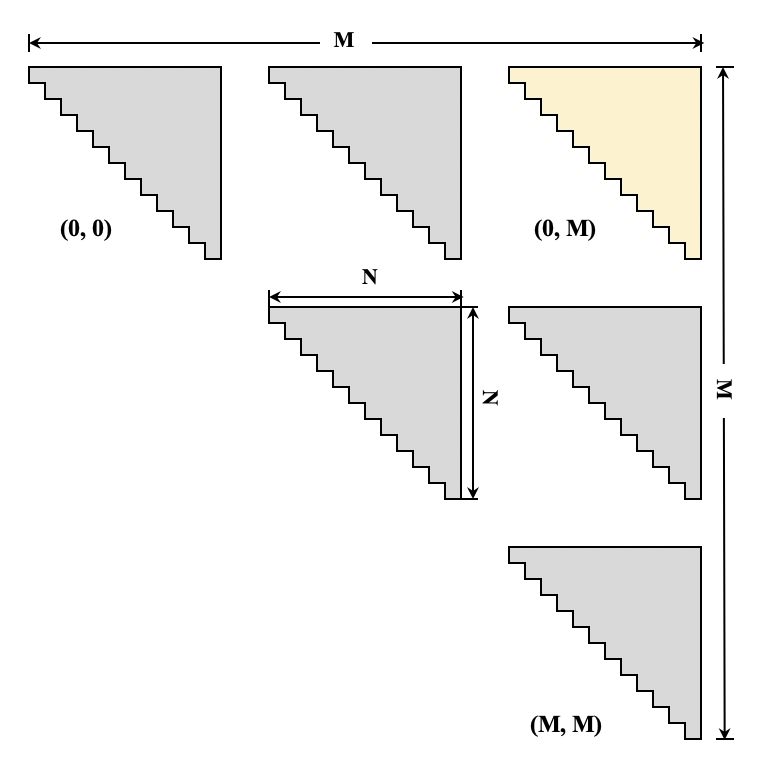
\includegraphics[scale=0.29, trim=2 2 2 2,clip]{content/figures/tile_0.png}
    \caption{FTable}
    \label{fig:tile_1}
    \end{subfigure}
    \begin{subfigure}[htbp]{0.22\linewidth}
    \centering
    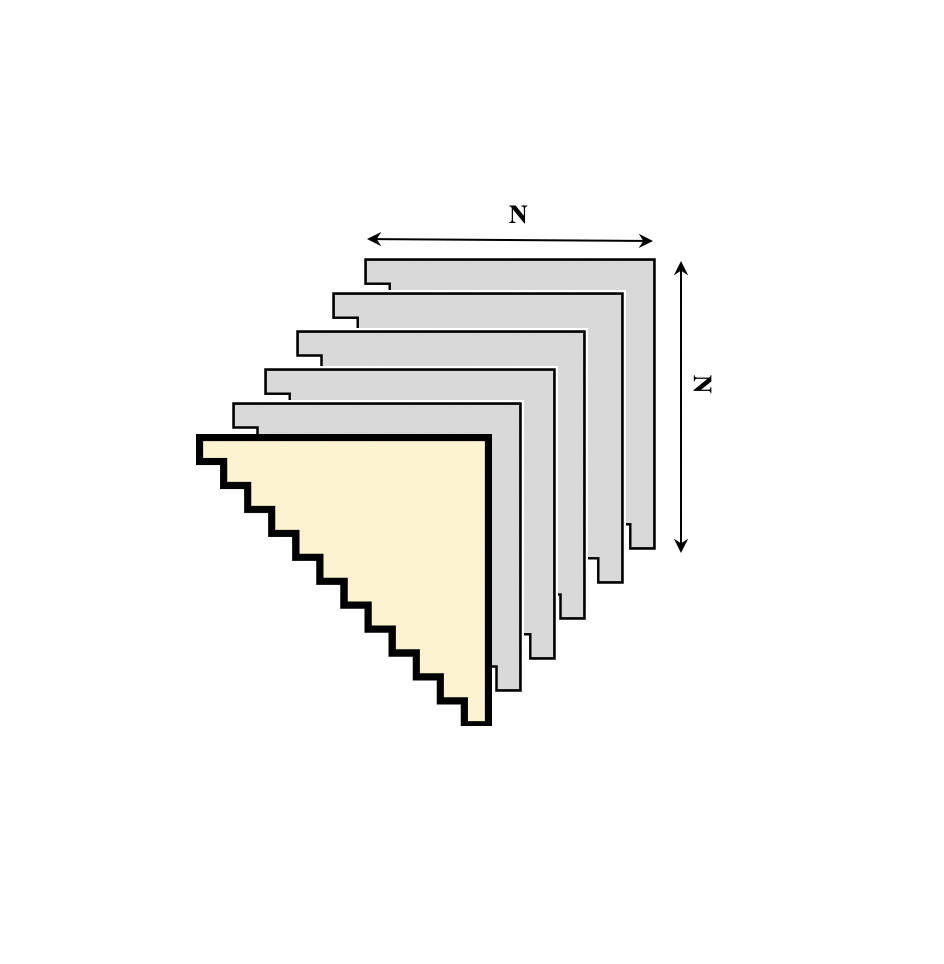
\includegraphics[scale=0.24, trim=2 2 2 2,clip]{content/figures/tile_1.png}
    \caption{Tile Level-I}
    \label{fig:tile_2}
    \end{subfigure}
    \begin{subfigure}[htbp]{0.22\linewidth}
    \centering
    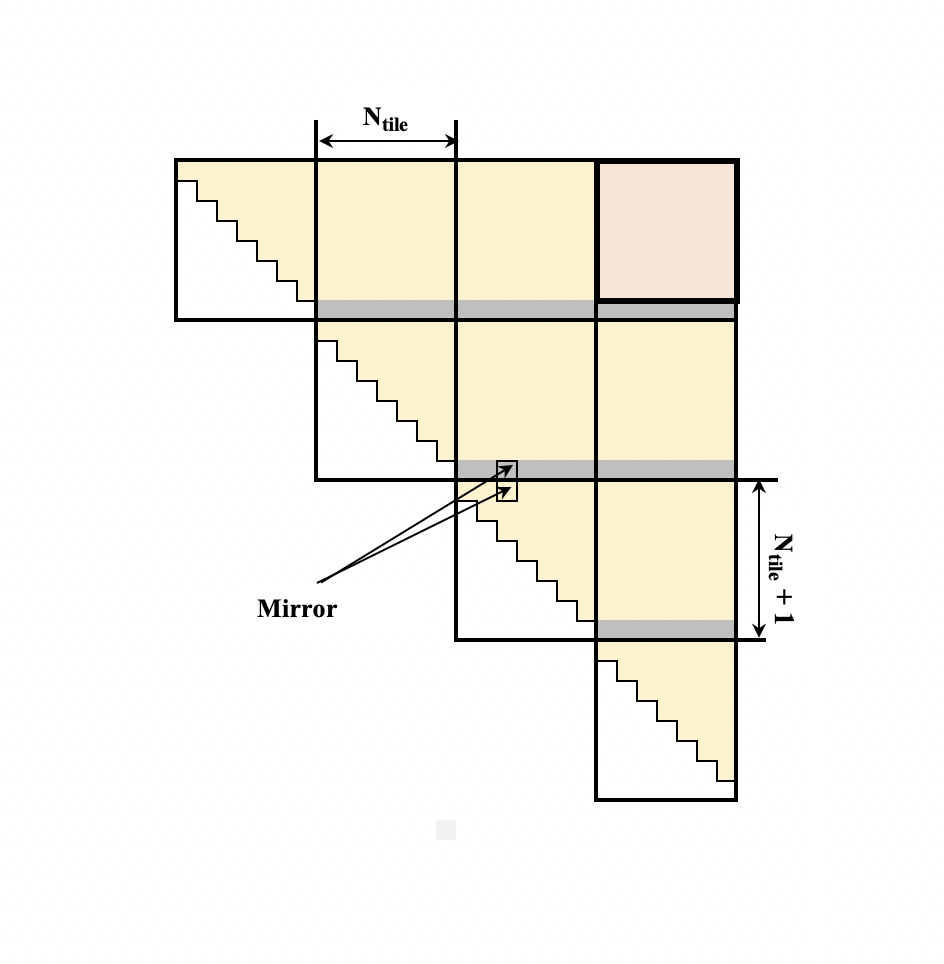
\includegraphics[scale=0.24, trim=2 2 2 2,clip]{content/figures/tile_2.png}
    \caption{Tile Level-II}
    \label{fig:tile_3}
    \end{subfigure}
    \begin{subfigure}[htbp]{0.22\linewidth}
    \centering
    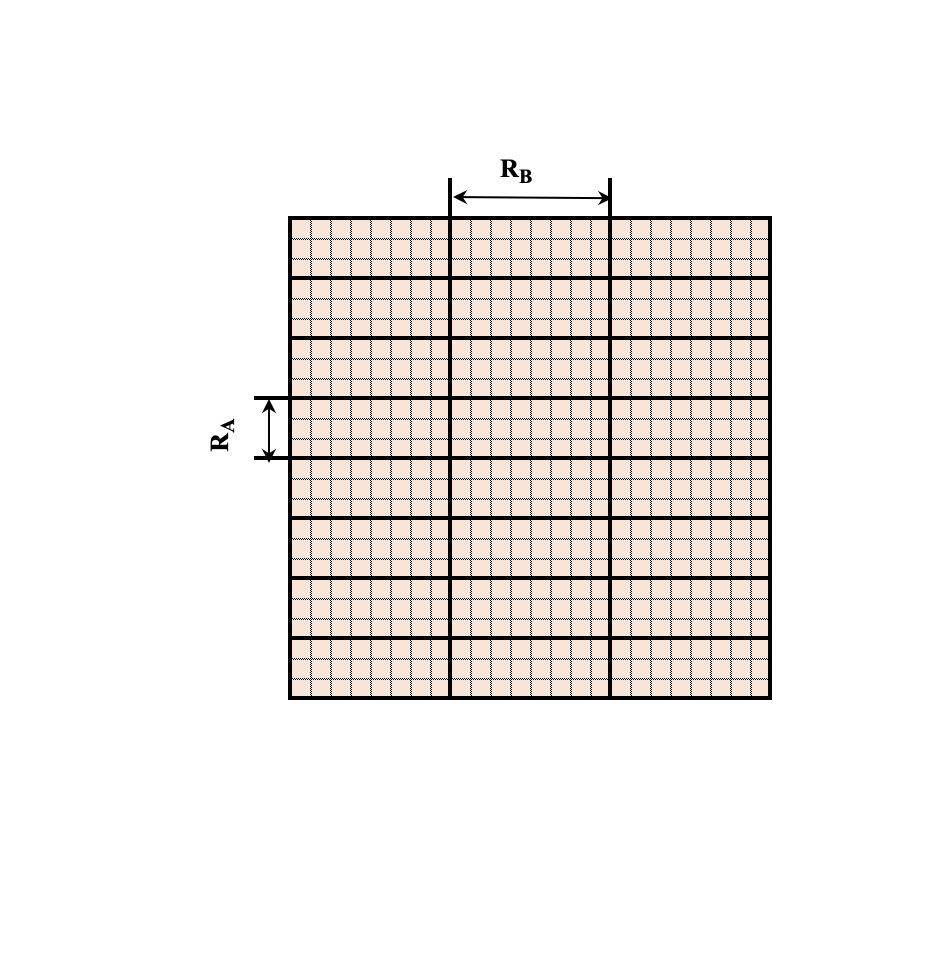
\includegraphics[scale=0.24, trim=2 2 2 2,clip]{content/figures/tile_3.png}
    \caption{Tile Level-III}
    \label{fig:tile_4}
    \end{subfigure}
\caption{Complete Tiling Overview: Computation granularity of the first-level tile ($N \times N$) is the inner triangle. The computation granularity of the second-level tile ($N_{tile+1} \times N_{tile}$) is the mono-parametric section of each inner triangle. Finally, the computation granularity of the third tiling level ($R_{A} \times R_{B}$) is the inner triangle subsection using registers.}
\label{fig:bpmax_full_tiling}
\end{figure*}

\subsubsection{Second-level Tiling : Mono-parametric Tiling (\textbf{MPT})}
The second-level tile divides the computation of each inner triangle based on a mono-parametric tile size with an aspect ratio of 1.  It takes an input parameter $N_{tile}$ as a program input and partitions each inner triangle into multiple sections/tiles ($N_{sec}$), where $N_{sec} =(N+N_{tile}-1) \div N_{tile}$,  $N$  = length of the second sequence (inner triangle). In other words, it introduces two new dimensions ($0 \le i_{2} \le j_{2} \le N_{sec}-1$ ) for each $F_{i_{1}, j_{1}, i_{22}, j_{22}}$ ($0 \le i_{1} \le j_{1} \le M$, $0 \le i_{22} \le j_{22} \le N$) and transforms it to $F_{i_{1}, j_{1}, i_{2}, j_{2}, i_{3}, j_{3}} (i_{22}, j_{22} \mapsto i_{2}, j_{2}, i_{3}, j_{3})$. This transformation allows us to decompose the computations easily and schedule them efficiently using our code generation tool. Now, all the second-level diagonal tiles are triangular since they represent the edge of the inner triangle. We add additional elements to these and make them rectangular. These elements are initialized to the max identity value ($MIN\_FLOAT$). Each non-diagonal tiles are two dimensional ($i_{3}, j_{3}$) rectangular matrices. We add a row to each one of these tiles ($i_{2}, j_{2}$) to copy the first row of the tile ($i_{2}+1, j_{2}$). Thus, the effective dimension of each one of the second-level tiles is $(N_{tile} +1) \times  N_{tile}$. It allows us to express all the BPMax reductions ($R^{0}, R^{1}, R^{2}, R^{3},$ and $R^{4}$) into many small matrix max-plus instances. Elements of each second-level tile are stored in row-major order, and the tiles themselves are stored in row-major order.

\begin{figure}
\centering
\begin{subfigure}[htbp]{0.48\textwidth}
\centering
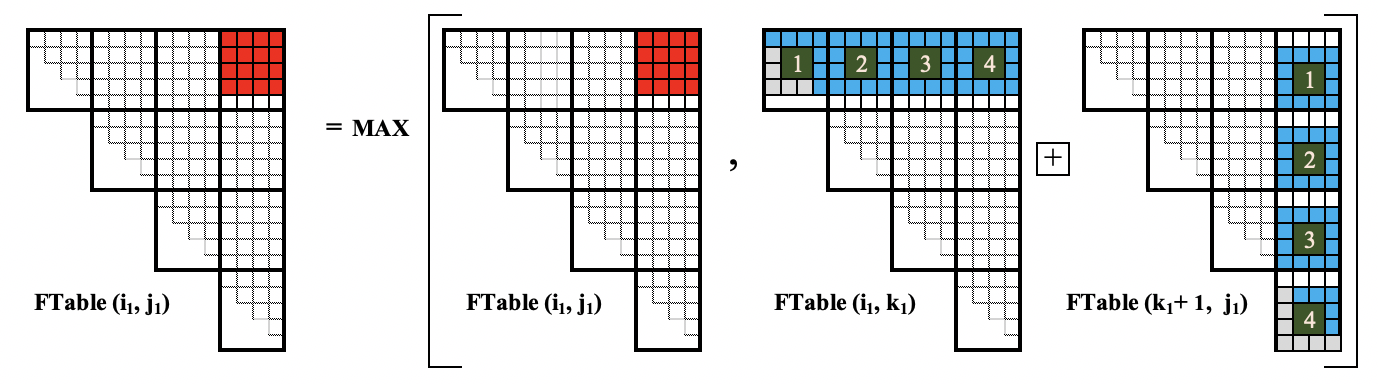
\includegraphics[scale=0.36, trim=4 4 4 4,clip]{content/figures/r0_mono_paramteric.png}
\caption{Second-level tiling of $R^{0}$}
\label{fig:mono_parametric_tile_r0}
\end{subfigure}
\hfill
\centering
\vspace{1mm}
\begin{subfigure}[htbp]{0.48\textwidth}
\centering
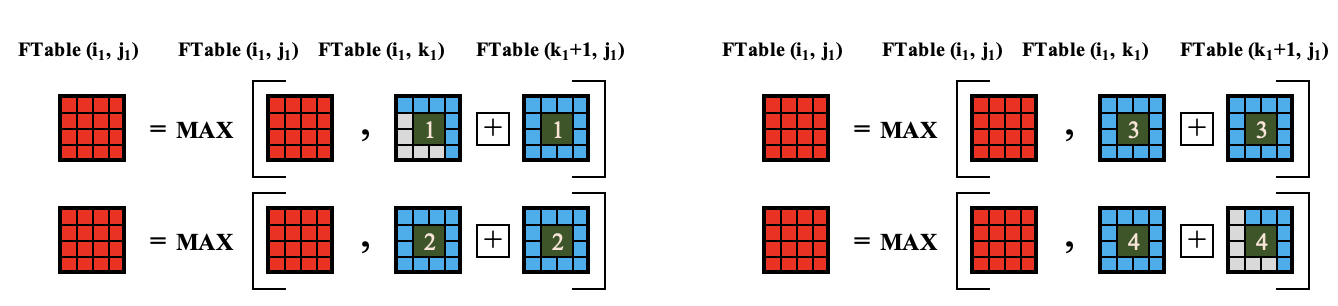
\includegraphics[scale=0.37, trim=4 4 4 4,clip]{content/figures/r0_max_plus.png}
\caption{Accumulation of $R^{0}$ using matrix max-plus}
\label{fig:matrix_max_plus_accum}
\end{subfigure}
\caption{Multi-level Decomposition of $R^{0}$}
\label{fig:rectangular_matrix_max_plus}
\end{figure}

\textbf{\textbf{MPT} of $R^{0}$:}
Mono-parametric tiling at the second-level transforms the original double max-plus into multiple matrix-plus operations.
Figure~\ref{fig:mono_parametric_tile_r0} shows a triangular matrix-max plus instance corresponding to a first-level tile, and Figure~\ref{fig:matrix_max_plus_accum} highlights the accumulation of a second-level tile (highlighted in red) using multiple small matrix max plus instances. The input and output tiles are distinct for each one of the second-level tiles. Thus, the processing order could be either any row-major or column-major, or even reverse. It is possible to either accumulate the results for each output tile or process one at a time. If we compute each tile at a time, all the input tiles are used only once for computing the output, resulting in poor data locality. We avoid this by partially accumulating results for a tile by reusing one of the matrices, which is implemented using a second-level tile schedule.



\textbf{\textbf{MPT} of $R^{3}$ and $R^{4}$:}
Mono-parametric tiling at the second-level for $R^{3}$ and $R^{4}$ is important since they use the same inner triangles used in $R^{0}$. These are element-wise operations between $R^{0}$ input tiles and $S_{1}$. $R^{0}$, $R^{3}$, and $R^{4}$ reductions share some input tiles for a given output tile. Equation~\ref{eqn:r3_recurrence_mono} and~\ref{eqn:r4_recurrence_mono} highlights recurrence for a second-level tile corresponding to $R^{3}$ and $R^{4}$. Tiling these computations at the second-level allows us to schedule the second-level tiles such that they share the same input tiles between $R^{0}$, $R^{3}$, and $R^{4}$ and improve data locality.
\begin{equation}
\label{eqn:r3_recurrence_mono}
R^{(3)}_{i_{1},j_{1},i_{2},j_{2}, i_{3}, j_{3}} = 
    \max\limits_{k_{2}=i_{1}}^{j_{1}-1} S_{i_{1},k_{1}} + F_{k_{1}+1,j_{1}, i_{2}, j_{2}, i_{3}, j_{3}}\\
\end{equation}
\begin{equation}
\label{eqn:r4_recurrence_mono}
R^{(4)}_{i_{1},j_{1},i_{2},j_{2}, i_{3}, j_{3}} = 
    \max\limits_{k_{2}=i_{1}}^{j_{1}-1}  F_{i_{1},k_{1}, i_{2}, j_{2}, i_{3}, j_{3}} + S_{k_{1}+1,j_{1}}\\
\end{equation}


\textbf{\textbf{MPT} of $R^{1}$ and $R^{2}$:}
One of the significant advantages of the new second-level tiling is that it enables the transformation of the two inner reductions $R^{1}$, and $R^{2}$ corresponding to $F(i_{1}, j_{1})$ that significantly reduces complex atomic updates highlighted in Figure~\ref{fig:final_ftable_update}. After applying the second-level tile, we observe that each output tile has inter-tile and intra-tile dependencies. The inter-tile dependencies can be resolved by processing the tiles diagonally or bottom-up, and the intra-tile dependencies can be resolved using $R^{1}$, and $R^{2}$. Notice that the majority of the $R^{1}$ and $R^{2}$ computations for each output tile can be transformed into several small matrix max-plus instances followed by a finalize phase that performs a small amount of $R^{1}$, and $R^{2}$. Like $R^{0}$ optimization, we can use a second-level tile schedule for these multiple matrices max-plus operations to reuse one of the inputs and partially accumulate results. 
\begin{figure}
\centering
\begin{subfigure}[b]{0.48\textwidth}
\centering
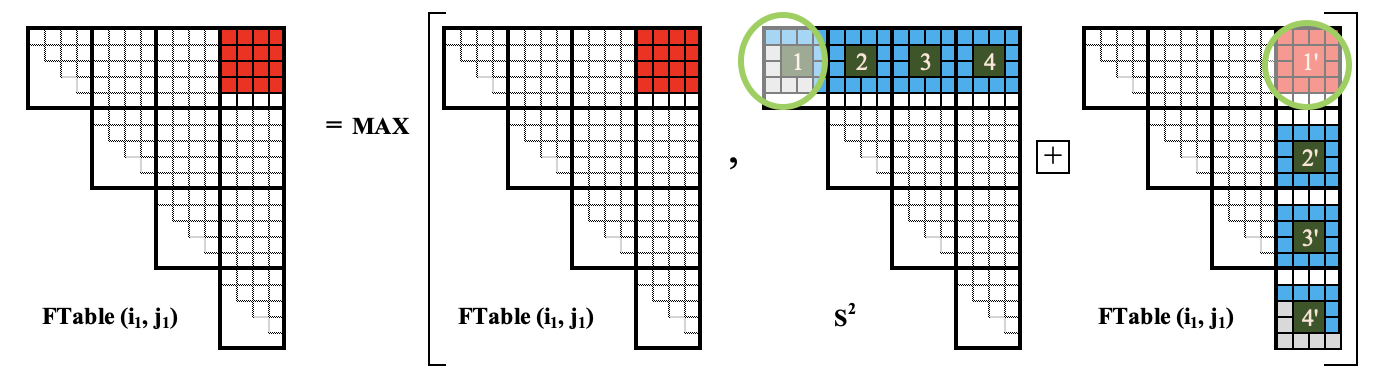
\includegraphics[scale=0.36, trim=4 4 4 4,clip]{content/figures/r1_top.png}
\label{fig:mono_r1_top}
\caption{Second-level Tiling of $R^{1}$}
\vspace{1mm}
\end{subfigure}
\centering
\begin{subfigure}[b]{0.48\textwidth}
\centering
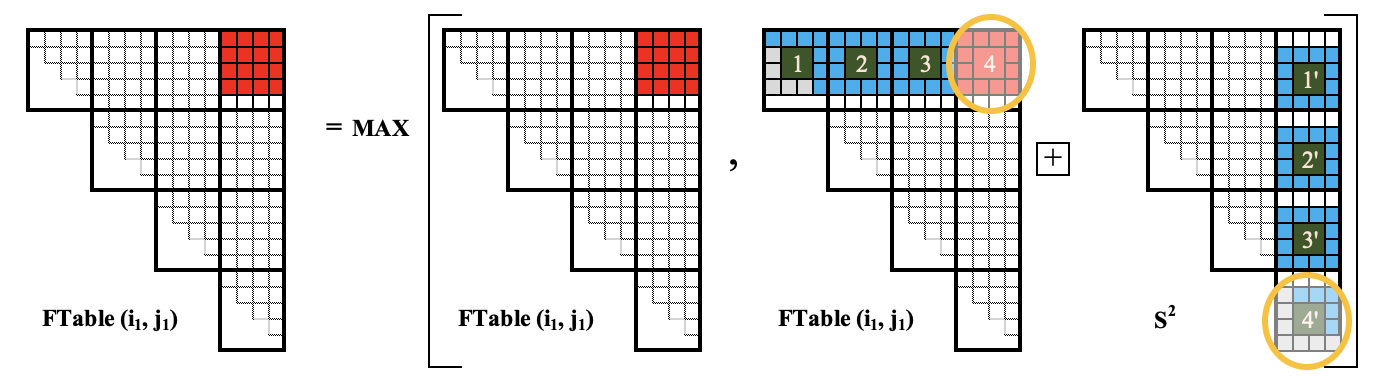
\includegraphics[scale=0.36, trim=4 4 4 4,clip]{content/figures/r2_top.png}
\caption{Second-level Tiling of $R^{2}$}
\label{fig:mono_r2_top}
\vspace{1mm}
\end{subfigure}
%\label{fig:r1_r2_optimization}
\begin{subfigure}[b]{0.22\textwidth}
\centering
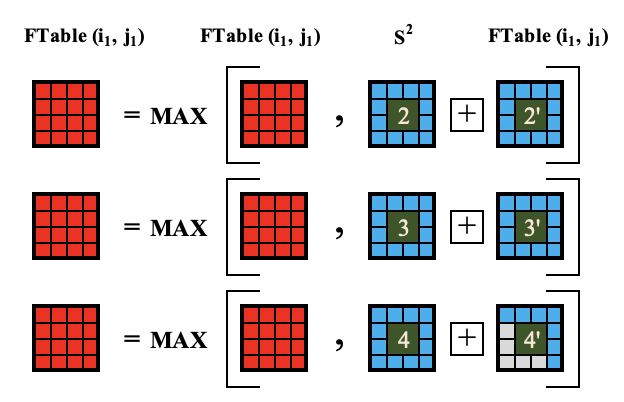
\includegraphics[width=\textwidth, scale=0.30, trim=4 4 4 4,clip]{content/figures/r1_max_plus.png}
\caption{$R^{1} \to$ Matrix max-plus}
\label{fig:R_1_matrix_max_plus}
\end{subfigure}
\vspace{0.5mm}
\begin{subfigure}[b]{0.22\textwidth}
\centering
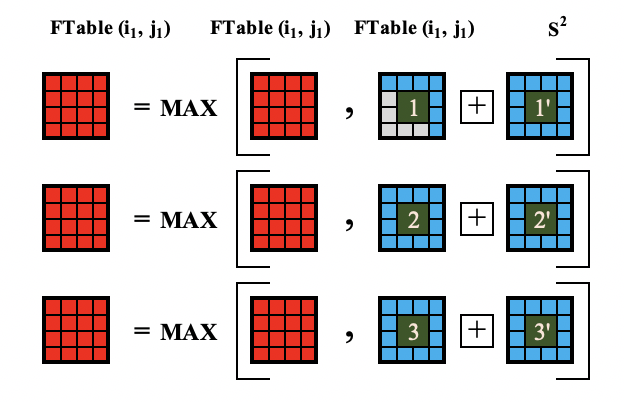
\includegraphics[width=\textwidth, scale=0.30, trim=4 4 4 4,clip]{content/figures/r2_max_plus.png}
\caption{$R^{2} \to$ Matrix max-plus}
\label{fig:R_2_matrix_max_plus}
\end{subfigure}
\begin{subfigure}[t]{0.22\textwidth}
\centering
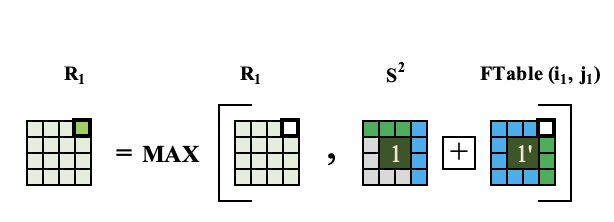
\includegraphics[width=\textwidth, scale=0.30, trim=4 4 4 4,clip]{content/figures/r1_finalize.png}
\caption{Residual $R^{1}$ }
\label{fig:mono_R_1}
\end{subfigure}
\begin{subfigure}[t]{0.22\textwidth}
\centering
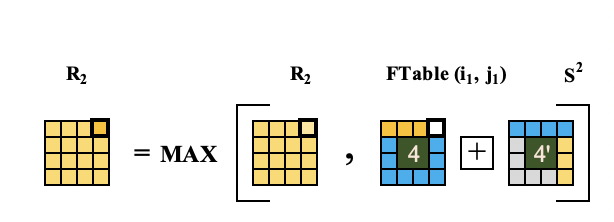
\includegraphics[width=\textwidth, scale=0.30, trim=4 4 4 4,clip]{content/figures/r2_finalize.png}
\caption{Residual $R^{2}$}
\label{fig:mono_R_2}
\end{subfigure}
\vspace{0.5mm}
\begin{subfigure}[t]{0.22\textwidth}
\centering
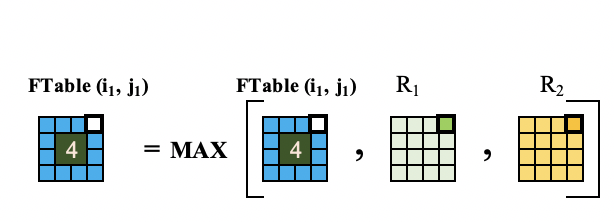
\includegraphics[width=\textwidth, scale=0.30, trim=4 4 4 4,clip]{content/figures/ftable_final.png}
\caption{Final Update}
\label{fig:mono_final}
\end{subfigure}
\caption{Multi-level Decomposition of $R^{1}$ and $R^{2}$}
\label{fig:R_1_2_matrix_max_plus}
\end{figure}
Besides the finalize phase, the diagonal tiles also require the $R^{1}$ and $R^{2}$ recurrences and use the same steps highlighted in Figure~\ref{fig:final_ftable_update}.
Figure~\ref{fig:R_1_2_matrix_max_plus} shows how a tile of $F(i_{1}, j_{1})$ is computed by transforming the computations into many small matrix max-plus problem instances and residual computations before making the final update.


\subsubsection{Third-level Tiling : Register Tiling (\textbf{RT})}

Second-level tiling allows us to improve data locality significantly. Now, we can rely on the vectorization process to improve CPU resource utilization and reduce L1 bandwidth by a factor of SIMD width. However, further optimization is required to reduce the L1 bandwidth and achieve maximum CPU utilization. So, we apply the register-blocking/tiling (\textbf{RT}), where we compute a patch (third-level tile) of the second-level tile that fits in the vector register. Elements from the input matrices are loaded into the memory and used multiple times to update the patch, effectively reducing the memory accesses for the input and output.

\begin{figure}[htbp]
\centerline{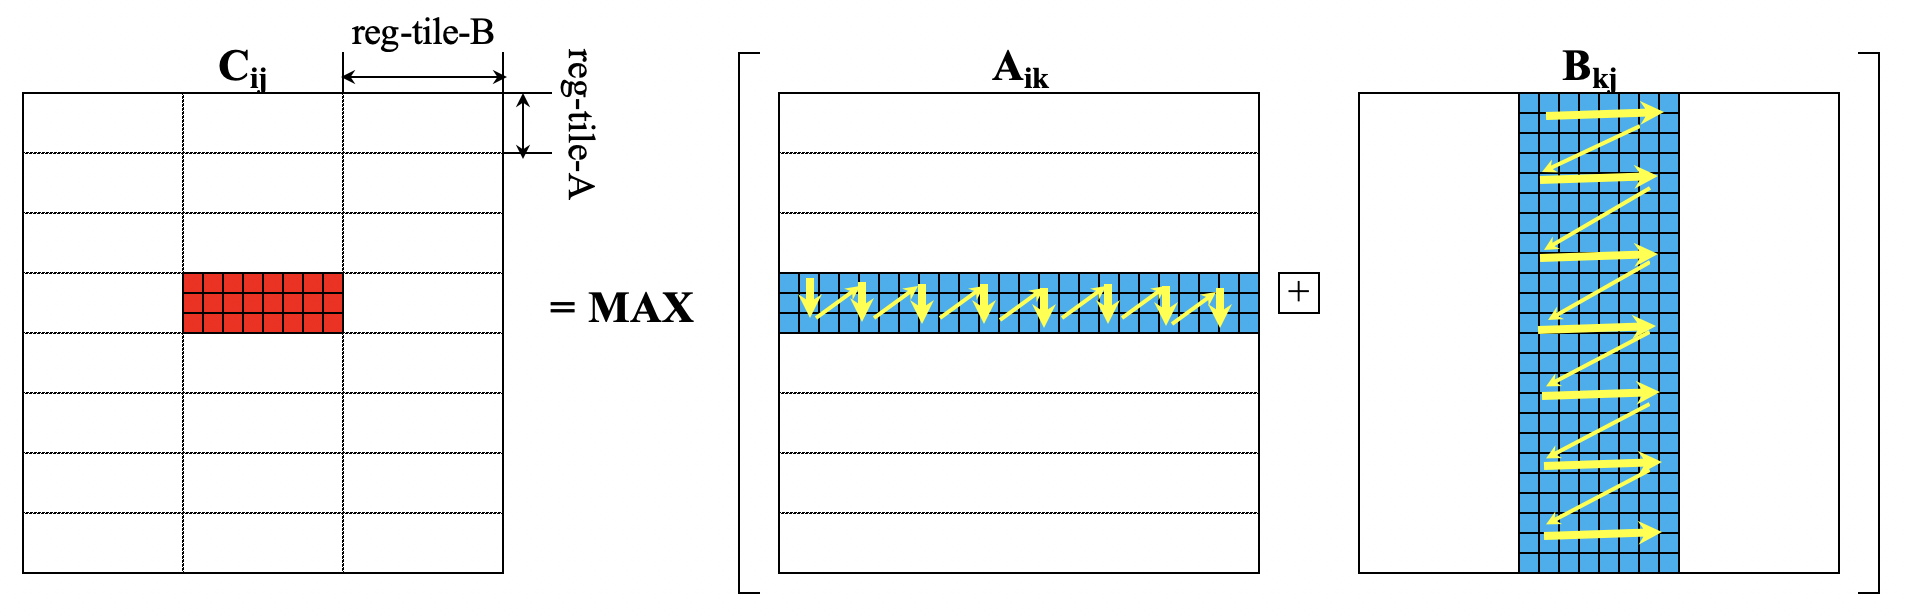
\includegraphics[scale=0.25, trim=5 5 5 5,clip]{content/figures/register_tile.png}}
\caption{Register Tiling (\textbf{RT})}
\label{fig:regiser_tile}
\end{figure}

Sequential memory access is a well-known property of any modern CPU-specific register-tiled kernel. Its performance depends on how the scalar and vector inputs are read from the memory and their alignments. So, we transform the first input matrix (let us call this A) and the second input matrix (let us call this B) such that the memory access pattern from the register-tile kernel is sequential. Figure~\ref{fig:regiser_tile} shows the memory access pattern of our register tile. Previously, similar techniques were also implemented for a register tile that performed FMA operations by Huang et al. \cite{FLAWN80}. We observe that an inner-$F$-table triangle or $S_{2}$ can be used several times as a $A$ or $B$ operand. Thus, it is possible to transform each triangle with two different memory layouts once and avoid transforming the same tile multiple times. 

\subsubsection{Buffer Transformation Strategy}
We have explored three buffer transformation techniques for accessing data sequentially within the register-tiled code. They are based on when we transform \textbf{register-tile-operand-A} and \textbf{register-tile-operand-format-B}. The first one \textbf{ [MPT+RT]:v1} transforms each inner $F$-table and $S_{2}$ to \textbf{register-tile-operand-A} and \textbf{register-tile-operand-format-B} exactly once but  introduces four new $F$-table variables - $F(A)$,  $F(B)$, $S_{2}(A)$, $S_{2}(B)$ in the system. The inner reductions $R_{1}$ and $R_{2}$ also use $S_{2}$ as the other operand for the max-plus operation. \textbf{ [MPT+RT]:v2} uses on-the-fly transformation for both of the operands, and \textbf{[MPT+RT]:v3} uses pre-transformed $S_{2}$ but transforms the inner $F$-table on the fly. 





\subsubsection{Parallelization Strategy} We process the first-level tiles diagonally and assign all the cores to a first-level tile to accumulate the results from each instance of outer reductions - $R^{0}$, $R^{3}$, and $R^{4}$. Each core is responsible for processing all the second-level tiles of a particular first-level tile. It helps the cores share the input and output inner triangles from the L3 cache. After all the first-level tiles in a diagonal are accumulated from outer reductions, we assign each core to update the first-level tile with the inner reductions - $R^{1}$, $R^{2}$. 




